\noindent Xét một khối trụ không đồng nhất được làm từ hai loại vật liệu có khối lượng riêng khác nhau. Khối trụ có bán kính $r$ và chiều dài $L$, mặt cắt của nó được minh hoạ trên hình 1.1. Nửa dưới được làm từ vật liệu có khối lượng riêng $1\,\text{kg/m}^3$ trong khi nửa trên được làm từ vật liệu có khối lượng riêng $c\,\text{kg/m}^3$ với $c$ là một tham số $0<c<1$. Biết rằng khối tâm của một bán trụ cso bán kính $r$ nằm cách trục đối xứng một đoạn $\dfrac{4r}{3\pi}$ như được chỉ ra trên hình 1.2.
\begin{figure}[h]
  \centering
  \begin{subfigure}[b]{0.49\textwidth}
    \centering
    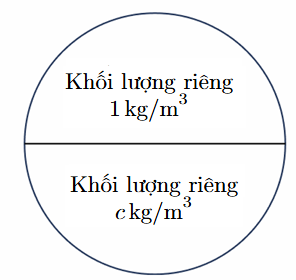
\includegraphics[width=0.65\textwidth]{Figures/Problems/Fig 1.1.png}
    \begin{center}
      \figurename{ 1.1}
    \end{center}
  \end{subfigure}
  \hfill
  \begin{subfigure}[b]{0.49\textwidth}
    \centering
    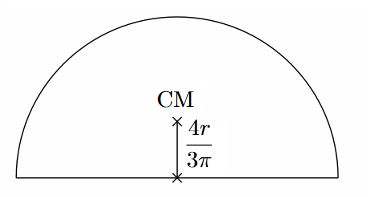
\includegraphics[width=0.75\textwidth]{Figures/Problems/Fig 1.2.png}
    \begin{center}
      \figurename{ 1.2}
    \end{center}
  \end{subfigure}
\end{figure}

\begin{enumerate}
  \item \begin{enumerate}
          \item Tính tổng khối lượng $M$ của khối trụ không đồng nhất và khoảng cách $d$ từ khối tâm của nó đến trục đối xứng theo $r, L$ và $c$.
          \item Tính momen quán tính $I$ của khối trụ đối với trục đối xứng theo $r, L$ và $c$.
        \end{enumerate}
  \item Trục đối xứng của khối trụ được gắn cố định nằm ngang và khối trụ có thể quay tự do không ma sát quanh trục đối xứng của nó. Xác định chu kì dao động bé của khối trụ quanh vị trí cân bằng theo $M, I, r, d$ và gia tốc trọng trường $g$.
\end{enumerate}
Bây giờ, khối trụ có thể di chuyển tự do trên mặt bàn nằm ngang dưới tác dụng của trọng lực. Giả sử hệ số ma sát trượt giữ khối trụ và mặt bàn là rất lớn, nhờ đó khối trụ luôn lăn không trượt. Tại $t=0$, khối trụ được thả ra từ vị trí cân bằng với tốc độ góc $\omega_0$.
\begin{enumerate}
  \setcounter{enumi}{2}
  \item \begin{enumerate}
          \item Nếu $\omega_0$ đủ nhỏ, khối trụ sẽ dao động quanh vị trí cân bằng của nó. Xác định chu kì dao động bé của khối trụ theo $M, I, r, d$ và $g$.
          \item Xác định giá trị nhỏ nhất của $\omega_0$ để khối trụ có thể lăn mãi mãi về một phía. Biểu diễn kết quả theo $M, I, r$ và $d$.
        \end{enumerate}
\end{enumerate}